\documentclass{article}% use option titlepage to get the title on a page of its own.
\usepackage[utf8]{inputenc}
\usepackage{amsmath} % allows us to type in math
\usepackage{verbatim} % allows us to type code like text
\usepackage{graphicx} % allows us to include figures
\usepackage{color}
\usepackage{float}
\usepackage{caption}
\usepackage{amssymb}
\usepackage{tikz}
\usepackage{pgfplots}
\usepackage{pgflibraryshapes}

\usetikzlibrary{arrows}
\pgfplotsset{compat=1.12}
\usetikzlibrary{patterns}

\title{Latex Reference}
\date{May 2020}
\author{Kyle Birnbaum}
\begin{document}
\maketitle

\begin{center}
    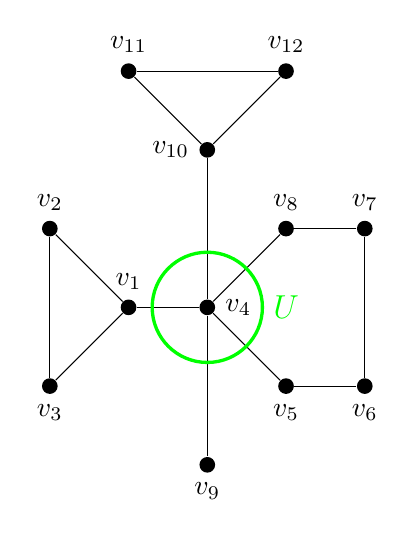
\begin{tikzpicture}
        \tikzset{vertex/.style = {circle,fill,inner sep=2pt}}
        \tikzset{edge/.style = {-,> = latex'}}

        \node[vertex, label=above:{$v_1$}] (v1) at (0,0) {};
        \node[vertex, label=above:{$v_2$}] (v2) at (-1,1) {};
        \node[vertex, label=below:{$v_3$}] (v3) at (-1,-1) {};
        \node[vertex, label=right:{$v_4$}] (v4) at (1,0) {};
        \node[vertex, label=below:{$v_5$}] (v5) at (2,-1) {};
        \node[vertex, label=below:{$v_6$}] (v6) at (3,-1) {};
        \node[vertex, label=above:{$v_7$}] (v7) at (3,1) {};
        \node[vertex, label=above:{$v_8$}] (v8) at (2,1) {};
        \node[vertex, label=below:{$v_9$}] (v9) at (1,-2) {};
        \node[vertex, label=left:{$v_{10}$}] (v10) at (1,2) {};
        \node[vertex, label=above:{$v_{11}$}] (v11) at (0,3) {};
        \node[vertex, label=above:{$v_{12}$}] (v12) at (2,3) {};

        \draw[edge] (v1) to (v2);
        \draw[edge] (v1) to (v3);
        \draw[edge] (v1) to (v4);

        \draw[edge] (v2) to (v3);

        \draw[edge] (v4) to (v5);
        \draw[edge] (v4) to (v8);
        \draw[edge] (v4) to (v9);
        \draw[edge] (v4) to (v10);

        \draw[edge] (v5) to (v6);

        \draw[edge] (v6) to (v7);

        \draw[edge] (v7) to (v8);

        \draw[edge] (v10) to (v11);
        \draw[edge] (v10) to (v12);

        \draw[edge] (v11) to (v12);

        \draw[color=green, very thick](1,0) circle (0.7);
        \node[color=green] at (2,0) {\large $U$};
    \end{tikzpicture}
\end{center}

\begin{center}
    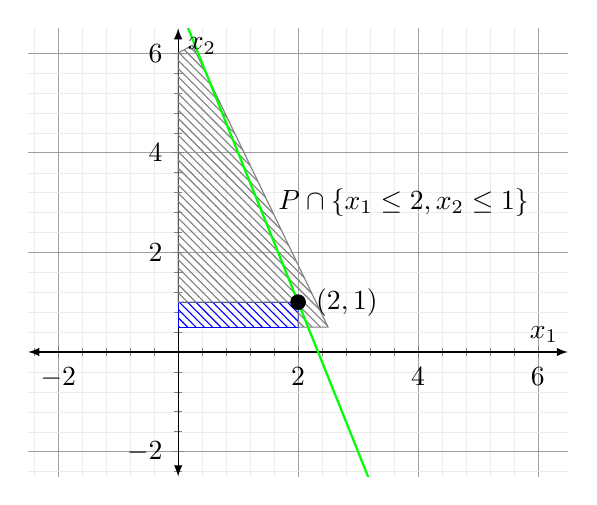
\begin{tikzpicture}
        \begin{axis}
            [
                xmin=-2,xmax=6, 
                ymin=-2,ymax=6,
                grid=both,
                grid style={line width=.1pt, draw=darkgray!10},
                major grid style={line width=.2pt,draw=darkgray!50},
                axis lines=middle,
                minor tick num=4,
                enlargelimits={abs=0.5},
                axis line style={latex-latex},
                samples=100,
                domain = -20:20,
                xlabel={$x_1$},
                ylabel={$x_2$}]
            ]
            % \addplot[red] {2*x/3 + 6};
            % \addplot[red] {-10*x/4 +27/4};
            % \addplot[red] {1/2};

            \filldraw[blue, pattern=north west lines, pattern color=blue] (0, 1/2) -- (2, 1/2) -- (2, 1)  -- (0, 1) -- cycle;
            \filldraw[gray, pattern=north west lines, pattern color=gray] (2, 1/2) -- (2,1) -- (0,1) -- (0,6) -- (9/38, 117/19) -- (5/2,1/2)-- cycle;
            \node[text width=4cm] at (axis cs:4.3,3) {$P \cap \{x_1 \leq 2, x_2 \leq 1\}$};
            
            
            \addplot[green, thick] {-3*x + 7};
            \node[label={right:{$(2,1)$}},circle,fill,inner sep=2pt] at (axis cs:2, 1) {};
            
        \end{axis}
    \end{tikzpicture}
\end{center}

\begin{center}
    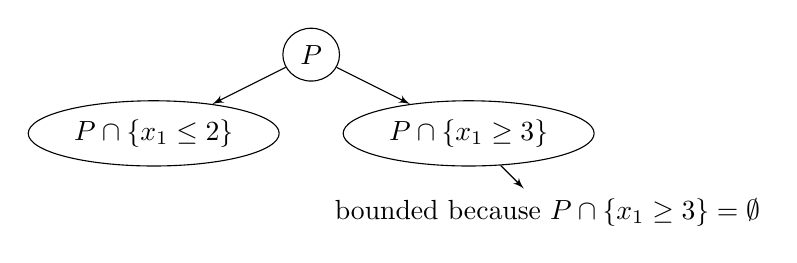
\begin{tikzpicture}
        \tikzset{vertex/.style = {shape=ellipse,draw,minimum size=1.5em}}
        \tikzset{label/.style = {minimum size=1.5em}}
        \tikzset{edge/.style = {->,> = latex'}}

        \node[vertex] (a) at (0,0) {$P$};
        \node[vertex] (b) at (-2,-1) {$P \cap \{x_1 \leq 2\}$};
        \node[vertex] (c) at (2,-1) {$P \cap  \{x_1 \geq 3\}$};
        \node[label] (d) at (3,-2) {bounded because $P \cap  \{x_1 \geq 3\} = \emptyset$};

        \draw[edge] (a) to node {} (b);
        \draw[edge] (a) to node {} (c);

        \draw[edge] (c) to node {} (d);
    \end{tikzpicture}
\end{center}

\begin{center}
    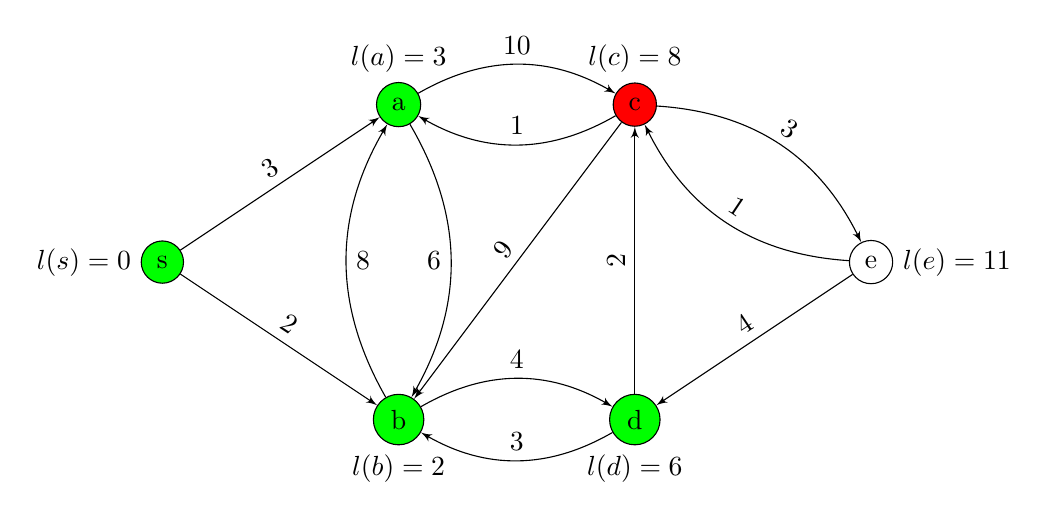
\begin{tikzpicture}
        \tikzset{vertex/.style = {shape=circle,draw,minimum size=1.5em}}
        \tikzset{edge/.style = {->,> = latex'}}
        % vertices
        \node[vertex, label=left:{$l(s) = 0$}, fill=green] (s) at (0,0) {s};
        \node[vertex, label={$l(a) = 3$}, fill=green] (a) at  (3,2) {a};
        \node[vertex, label=below:{$l(b) = 2$},fill=green] (b) at  (3,-2) {b};
        \node[vertex, label={$l(c) = 8$}, fill=red] (c) at  (6,2) {c};
        \node[vertex, label=below:{$l(d) = 6$}, fill=green] (d) at (6,-2) {d};
        \node[vertex, label=right:{$l(e) = 11$}] (e) at (9,0) {e};

        %edges
        \draw[edge] (s) to node[above, sloped] {3} (a);
        \draw[edge] (s) to node[above, sloped] {2} (b);
        \draw[edge] (c) to node[above, sloped] {9} (b);
        \draw[edge] (d) to node[above, sloped] {2} (c);
        \draw[edge] (e) to node[above, sloped] {4} (d);
        
        \draw[edge] (a)  to[bend left] node[left] {6} (b);
        \draw[edge] (b) to[bend left] node[right] {8} (a);

        \draw[edge] (a)  to[bend left] node[above, sloped] {10} (c);
        \draw[edge] (c) to[bend left] node[above, sloped] {1} (a);

        \draw[edge] (b) to[bend left] node[above, sloped] {4} (d);
        \draw[edge] (d)  to[bend left] node[above, sloped] {3} (b);

        \draw[edge] (c) to[bend left] node[above, sloped] {3} (e);
        \draw[edge] (e)  to[bend left] node[above, sloped] {1} (c);
    \end{tikzpicture}
\end{center}

\end{document}